\chapter{Approximate Bayesian Computing}

Let $(\theta_i)_{i\in \{1,\dots, n\}}$ be a set of parameters with prior distribution $\pi$, and $(x_j)_{j\in \{1,\dots, m\}}$ be the set of realised data, generated using $(\theta_i)_{i\in \{1,\dots, n\}}$. The most basic approximate Bayesian computation algorithm is such:
\texttt{\\
    1. Generate $(\hat{\theta_i})_{i\in \{1,\dots, n\}}\sim \pi$\\
    2. Using $(\theta_i)_{i\in \{1,\dots, n\}}$, regenerate the data $(\hat{x_j})_{j\in \{1,\dots, m\}}$ using the\\ parameter set $(\hat{\theta_i})_{i\in \{1,\dots, n\}}$\\
    3. If $(\hat{x_j})_{j\in \{1,\dots, m\}} = (x_j)_{j\in \{1,\dots, m\}}$, accept $(\hat{\theta_i})_{i\in \{1,\dots, n\}}$, else regenerate\\ $(\hat{\theta_i})_{i\in \{1,\dots, n\}}$ and go to step 2
}

For non-discrete cases

Generate parameter(s) from your prior.

Generate the data.

If it matches (or is close enough), add that parameter to your set of accepted parameters. This set will approximate the posterior distribution.

Drawbacks of this approach. Very difficult to estimate multiple parameters to the one outcome parameters. Or if you have a single parameter, generating multiple observations, unlikely to match all of them. Same with multiple parameters to multiple outputs

\begin{figure}
    \centering
    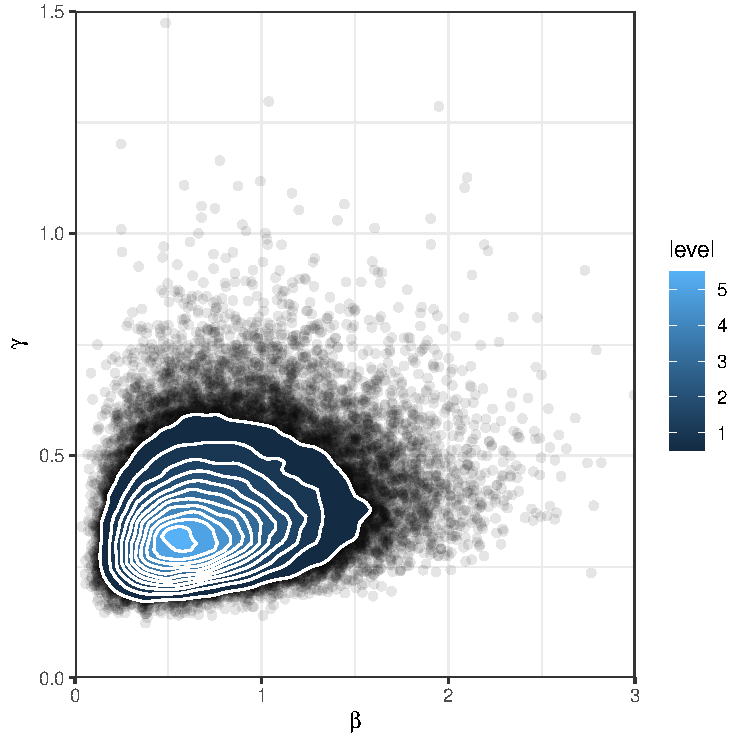
\includegraphics{SIS_ABC.pdf}
    \caption{Using a basic SIS model as in previous figure using ABC to generate from posterior beta, gamma}
    \label{fig:ABC_R}
\end{figure}

\section{Summary Statistics}

\subsection*{Distribution of summary statistic}

Should be relatively normally distributed

\section{Discrepency}

\subsection*{Distribution of discrepency}

|Normal - normal| or something so should be normalish?

\section{Estimating the likelihood from the summary statistic}